%%%%%%%% ICML 2023 EXAMPLE LATEX SUBMISSION FILE %%%%%%%%%%%%%%%%%

\documentclass{article}

% Recommended, but optional, packages for figures and better typesetting:
\usepackage{microtype}
\usepackage{graphicx}
% \usepackage{subfigure}
\usepackage{booktabs} % for professional tables
\usepackage{multirow}

% hyperref makes hyperlinks in the resulting PDF.
% If your build breaks (sometimes temporarily if a hyperlink spans a page)
% please comment out the following usepackage line and replace
% \usepackage{icml2023} with \usepackage[nohyperref]{icml2023} above.
\usepackage{hyperref}

% Plots
% \usepackage{tikz}
% \usepackage{pgfplots}
% \pgfplotsset{compat=1.15}
% \usepgfplotslibrary{fillbetween}
% \usetikzlibrary{external}
\usepackage{tikz}
\usepackage{pgfplots}
\usepgfplotslibrary{fillbetween}
\usepackage{subcaption}


% Attempt to make hyperref and algorithmic work together better:
\newcommand{\theHalgorithm}{\arabic{algorithm}}

% Use the following line for the initial blind version submitted for review:
\usepackage{icml2023}

% If accepted, instead use the following line for the camera-ready submission:
% \usepackage[accepted]{icml2023}

% For theorems and such
\usepackage{units}
\usepackage{amsmath}
\usepackage{amssymb}
\usepackage{mathtools}
\usepackage{amsthm}

% if you use cleveref..
\usepackage[capitalize,noabbrev]{cleveref}

%%%%%%%%%%%%%%%%%%%%%%%%%%%%%%%%
% THEOREMS
%%%%%%%%%%%%%%%%%%%%%%%%%%%%%%%%
\theoremstyle{plain}
\newtheorem{theorem}{Theorem}[section]
\newtheorem{proposition}[theorem]{Proposition}
\newtheorem{lemma}[theorem]{Lemma}
\newtheorem{corollary}[theorem]{Corollary}
\theoremstyle{definition}
\newtheorem{definition}[theorem]{Definition}
\newtheorem{assumption}[theorem]{Assumption}
\theoremstyle{remark}
\newtheorem{remark}[theorem]{Remark}

% Todonotes is useful during development; simply uncomment the next line
%    and comment out the line below the next line to turn off comments
%\usepackage[disable,textsize=tiny]{todonotes}
\usepackage[textsize=tiny]{todonotes}







% macros
\newcommand*{\VEC}[1]  {\ensuremath{\boldsymbol{#1}}}
\newcommand*{\MAT}[1]  {\ensuremath{\boldsymbol{#1}}}


\newcommand*{\nfeatures}{\ensuremath{p}}
\newcommand*{\nsamples}{\ensuremath{n}}
\newcommand{\nc}{\ensuremath{c}}


\newcommand*{\realSpace}{\ensuremath{\mathbb{R}}}
\newcommand*{\SymSpace}{\ensuremath{\mathcal{S}_{\nfeatures}}}
\newcommand*{\DiagSpace}{\ensuremath{\mathcal{D}_{\nfeatures}}}
\newcommand*{\SPDman}{\ensuremath{\mathcal{S}^{++}_{\nfeatures}}}
\newcommand*{\DPDman}{\ensuremath{\mathcal{D}^{++}_{\nfeatures}}}


\newcommand*{\eye}{\ensuremath{\MAT{I}_{\nfeatures}}}
\newcommand*{\onevec}{\ensuremath{\VEC{1}_{\nfeatures}}}


\newcommand*{\Cov}{\ensuremath{\MAT{C}}}
\newcommand*{\SCM}{\ensuremath{\MAT{\hat{C}}}}
\newcommand*{\linearLW}{\ensuremath{\MAT{\hat{C}}_{\textup{LW}}}}
\newcommand*{\nonlinearLW}{\ensuremath{\MAT{\hat{C}}_{\textup{LW-NL}}}}
\newcommand*{\CovRMTdist}{\ensuremath{\MAT{\hat{C}}_{\textup{dist}}}}

\newcommand*{\Mean}{\ensuremath{\MAT{G}}}


\newcommand*{\point}{\ensuremath{\MAT{R}}}

\newcommand*{\eigsMat}{\ensuremath{\MAT{\Lambda}}}


\newcommand*{\tangentVector}{\ensuremath{\boldsymbol{\xi}}}
\newcommand*{\tangentVectorBis}{\ensuremath{\boldsymbol{\eta}}}


\newcommand*{\RMTdistSCMdeter}{\ensuremath{\hat{\delta}^2}}
\newcommand*{\RMTdistSCMs}{\ensuremath{\tilde{\delta}^2}}






\newcommand*{\dataCov}{\ensuremath{\VEC{x}_i}}
\newcommand*{\nsamplesCov}{\ensuremath{\nsamples_x}}
\newcommand{\ncCov}{\ensuremath{\nc_x}}




\newcommand*{\SCMIterate}{\ensuremath{\MAT{\hat{M}}}}
\newcommand*{\dataIterate}{\ensuremath{\VEC{y}_i}}
\newcommand*{\nsamplesIterate}{\ensuremath{\nsamples_y}}
\newcommand{\ncIterate}{\ensuremath{\nc_y}}


\newcommand*{\Stieltjes}{\ensuremath{m_{\mu}}}

\DeclareMathOperator{\tr}{tr}
\DeclareMathOperator{\diff}{d}
\DeclareMathOperator{\symm}{sym}
\DeclareMathOperator{\diag}{diag}
\DeclareMathOperator*{\argmin}{argmin}
% \DeclareMathOperator{\grad}{grad}

\newcommand*{\grad}{\ensuremath{\nabla}}

\newcommand*{\dataMat}{\ensuremath{\MAT{X}}}










% The \icmltitle you define below is probably too long as a header.
% Therefore, a short form for the running title is supplied here:
\icmltitlerunning{Frechet-Karcher Mean with low sample support: exploiting random matrix theory and Riemannian geometry}

\begin{document}

\twocolumn[
\icmltitle{Fréchet-Karcher Mean with low sample support: \\ exploiting random matrix theory and Riemannian geometry}

% It is OKAY to include author information, even for blind
% submissions: the style file will automatically remove it for you
% unless you've provided the [accepted] option to the icml2023
% package.

% List of affiliations: The first argument should be a (short)
% identifier you will use later to specify author affiliations
% Academic affiliations should list Department, University, City, Region, Country
% Industry affiliations should list Company, City, Region, Country

% You can specify symbols, otherwise they are numbered in order.
% Ideally, you should not use this facility. Affiliations will be numbered
% in order of appearance and this is the preferred way.
\icmlsetsymbol{equal}{*}

\begin{icmlauthorlist}
\icmlauthor{Florent Bouchard}{equal,l2s}
\icmlauthor{Ammar Mian}{listic}
\icmlauthor{Malik Tiomoko}{equal,huawei}
\icmlauthor{Guillaume Ginolhac}{listic}
\icmlauthor{Frédéric Pascal}{l2s}
\end{icmlauthorlist}

\icmlaffiliation{huawei}{Huawei Paris Research Center}
\icmlaffiliation{l2s}{Université Paris Saclay, CNRS, CentraleSupélec, L2S}
\icmlaffiliation{listic}{Université Savoie Mont Blanc, LISTIC}

\icmlcorrespondingauthor{Malik Tiomoko}{??}
\icmlcorrespondingauthor{Florent Bouchard}{florent.bouchard@cnrs.fr}

% You may provide any keywords that you
% find helpful for describing your paper; these are used to populate
% the "keywords" metadata in the PDF but will not be shown in the document
\icmlkeywords{Random matrix theory, covariance matrices, Karcher mean, Riemannian geometry}

\vskip 0.3in
]

% this must go after the closing bracket ] following \twocolumn[ ...

% This command actually creates the footnote in the first column
% listing the affiliations and the copyright notice.
% The command takes one argument, which is text to display at the start of the footnote.
% The \icmlEqualContribution command is standard text for equal contribution.
% Remove it (just {}) if you do not need this facility.

%\printAffiliationsAndNotice{}  % leave blank if no need to mention equal contribution
\printAffiliationsAndNotice{\icmlEqualContribution} % otherwise use the standard text.

\begin{abstract}
    In this paper, THE new standard way to learn covariance matrices with low sample support is proposed.
    To do so, two very powerful tools are leveraged: the random matrix theory (RMT) and Riemannian geometry.
\end{abstract}


\section{Introduction}

\begin{itemize}
    \item Computation of Karcher Mean (KM) from $K$ SPD matrices. This algorithm does not have a close form and so iterative algorithms. Everything ok in theorey. But in real life covariance are shitty and so the KM can be impossible to compute
    \item One solution : the regularazitation !!!
    \begin{itemize}
        \item MoT Shrink to identity. Depends on one or two parameters. 
        \item To find the best parameters, we have to choose a criteria. In literature it is MSE, whitening, oracle, ... Not connected to the application (execpt paper of fred, romain, abla, max pd).
        \item The best of the best is LW Non Linear
        \item Other issues: the regul is only on the eigenvalues
        \item In 2019, we propose to regularize by using a distance. More convenient for classif. Ok but some issues        
    \end{itemize}
    \item In this paper, we propose a new estimator without the issue
    \item But most important a new KM because better to do regul by taking into account the appli ! Actually barycenters are useful in ML for MDM, K-Means or batchnorm (brooks neurips). 
    \item Some references using KM in ML : \cite{utpala2023,lou2020}. Even use for privacy \cite{reimherr2021}. For metric learning \cite{zadeh2016}. For SPD deep network \cite{brooks2019riemannian}.
\end{itemize}

\section{Preliminaries}

\subsection{Random matrix theory}
\subsubsection{Background}
Random matrix theory (RMT) is a tremendous tool when it comes to studying the statistical properties of random matrices when the number of samples $\nsamples$ is not that greater than the number of features $\nfeatures$.
%
RMT comes from the pioneering work~\cite{wishart1928generalised}, which aimed at studying the eigenvalues of the so-called Wishart matrix $\dataMat\dataMat^T$, where $\dataMat\in\realSpace^{\nfeatures\times\nsamples}$, with  each element $\dataMat_{ij}$ drawn from the normal distribution $\mathcal{N}(0,1)$ with zero mean and unit variance.
Great improvements for the study of the spectral distribution of Wishart matrices were then obtained in~\cite{marchenko1967distribution}.
It heavily relies on the independance of the samples and on the Stieltjes transform of the empirical spectral distribution $\mu_{\nfeatures}=\frac1\nfeatures\sum_{i=1}^\nfeatures\delta_{\lambda_i(\SCM)}$ of the sample covariance matrix (SCM) $\SCM=\frac1\nsamples\dataMat\dataMat^T$, given by
\begin{equation*}
    \frac1\nfeatures\tr((\frac1\nsamples\dataMat\dataMat^T - z\eye)^{-1})
    =
    \int (\lambda-z)^{-1}\mu_{\nfeatures}(dt).
\end{equation*}
These results were then extended in~\cite{silverstein1995empirical,bai1998no}, which contain a thorough study of sample covariance matrices.
These indeed provide a random matrix result relating directly the limiting eigenvalue distributions of the sample covariance matrix $\SCM$ and the true covariance $\Cov$.

From a practical point of view, given $\dataMat\in\realSpace^{\nfeatures\times\nsamples}$ drawn from a normal distribution with true covariance matrix $\Cov\in\SPDman$,  works~\cite{silverstein1995empirical,bai1998no} yielded a strong hope to improve the estimation of the true eigenvalues $\lambda_i(\Cov)$  with RMT.
However, even though estimating $\lambda_i(\SCM)$ from $\lambda_i(\Cov)$ is easy, the other way around, \emph{i.e.}, estimating $\lambda_i(\Cov)$ from $\lambda_i(\SCM)$, is quite difficult with a limited number of samples $\nsamples$.
%
A simple idea~\cite{ledoit2004well} consists in linearly shrinking $\SCM$ with $\linearLW=\rho\eye + \sqrt{1-\rho^2}\SCM$, where $\rho>0$ is chosen so that it minimizes the expected $\ell2$ distance $\mathbb{E}[\| \Cov - \linearLW \|_2]$ asympotically, \emph{i.e.}, $\nfeatures,\nsamples\to\infty$ with $\nfeatures/\nsamples\to\nc>0$.
To estimate $\rho$ consistently, basic results from RMT are used.
However, in this setting, we are actually far from estimating the true eigenvalues $\lambda_i(\Cov)$.
%
A great step in that direction was then proposed in~\cite{mestre2008asymptotic}.
Thanks to contour integrals, it consistently estimates linear functions $\frac1\nsamples\sum_{i=1}^\nsamples f(\lambda_i(\Cov))$ from the $\lambda_i(\SCM)$'s.
Unfortunately, $f$ needs to be very smooth so the $\lambda_i(\Cov)$'s cannot be evaluated individually.
%
In~\cite{ledoit2015spectrum} and~\cite{ledoit2018optimal}, the $\ell2$ distance and a Stein loss are leveraged to estimate the $\lambda_i(\Cov)$'s from the $\lambda_i(\SCM)$'s with the so-called QuEST method.
The major limitation is that, even though QuEST is quite accurate, it is computationnally very expensive, which makes it complicated to employ in real scenarios.
%
Recently, \cite{ledoit2020analytical} proposed an analytical non-linear shrinkage of the $\lambda_i(\SCM)$'s, \emph{i.e.}, functions $\phi_i$ are learnt such that the $\lambda_i(\Cov)$'s are estimated through $\phi_i(\lambda_i(\SCM))$.
To determine the $\phi_i$'s, RMT, oracle non-linear shrinkage function and kernels are exploited.
They are chosen to minimize the true variance.
This method features the accuracy of QuEST while being numerically very efficient.

\subsubsection{Distance estimation}
\label{sec:preliminaries:RMT_dist}
Covariance matrices are at the core of many machine learning techniques, such as linear and quadratic discriminant analysis, metric learning, \emph{etc}.
Hence, RMT has attracted some attention in the machine learning community, even beyond covariances.
The reader is referred to~\cite{couillet2022random} for a recent textbook treating the subject (including kernels, support vector machine  or neural networks).
In the present paper, we focus on learning methods that rely on distances between covariance matrices, such as the nearest centroid classifier or K-means.
We are thus very interested in accurately estimating such distances.


In~\cite{couillet2019random,pereira2023consistent}, RMT corrected estimators of the squared distance between the true covariance matrices of some data are derived.
In both cases, given two data matrices $\dataMat_1\in\realSpace^{\nfeatures\times\nsamples_1}$ and $\dataMat_2\in\realSpace^{\nfeatures\times\nsamples_2}$, consistent estimators $\RMTdistSCMs(\SCM_1,\SCM_2)$ of the squared distance $\delta^2(\Cov_1,\Cov_2)$ between their true covariance $\Cov_1$ and $\Cov_2$ are provided.
In~\cite{couillet2019random}, results are provided for any squared distance function that only depends on the eigenvalues of $\Cov_1^{-1}\Cov_2$.
Applications to the Kullback-Leibler divergence, Bhattacharyya and Fisher distances are given.
In~\cite{pereira2023consistent}, an extension to handle the log-Euclidean distance, which does not depend on the eigenvalues of $\Cov_1^{-1}\Cov_2$, is obtained.
In both papers, derivations strongly rely on Stieltjes transforms and therefore involve the computation of very complicated contour integrals.
Fortunately, authors still managed to obtain closed form expressions for all considered distances.
%
In~\cite{couillet2019random}, given $\dataMat\in\realSpace^{\nfeatures\times\nsamples}$, authors further provided a consistent estimator $\RMTdistSCMdeter(\point,\SCM)$ of the squared distance $\delta^2(\point,\Cov)$ between the true covariance $\Cov$ and a deterministic $\point\in\SPDman$. 
%
Since they exploit the results from~\cite{silverstein1995empirical}, one very important thing to bare in mind is that these RMT corrected distance estimators are relevant only if $\dataMat_1$ and $\dataMat_2$ are independent (respectively that $\point$ is not constructed with $\dataMat$).


We focus on the squared Fisher distance~\cite{skovgaard1984riemannian}, which is given by
\begin{equation}
    \begin{array}{rcl}
        \delta^2(\Cov_1,\Cov_2) & = & \frac1{2\nfeatures}\| \log(\Cov_1^{-1}\Cov_2) \|_2^2  \\
         & = & \frac1{2\nfeatures}\sum_{i=1}^{\nfeatures} \log^2(\lambda_i(\Cov_1^{-1}\Cov_2)).
    \end{array}
\label{eq:Fisher_dist}
\end{equation}
% Given $\dataMat_1\in\realSpace^{\nfeatures\times\nsamples_1}$ and $\dataMat_2\in\realSpace^{\nfeatures\times\nsamples_2}$, the correction advocated in~\cite{couillet2019random} is
% \begin{multline}
%     \RMTdistSCMs(\SCM_1,\SCM2) = \frac1{2\nfeatures}\sum_{i=1}^{\nfeatures} \log^2((1-\nc_1)\lambda_i)
%     - \frac1\nfeatures(\VEC{\eta}-\VEC{\zeta})^T\MAT{N}\onevec
%     \\
%     - \frac{1-\nc_2}{\nc2}[ (\VEC{\eta}-\VEC{\zeta})^T\VEC{r} + \frac12\log^2((1-\nc_1)(1-\nc_2)) ]
%     \\
%     + (\frac{\nc_1+\nc_2}{\nc_1\nc2}-1)(\VEC{\eta}-\VEC{\lambda})^T[ \MAT{M}^T(\VEC{\eta}-\VEC{\zeta}) + \VEC{r}  ],
% \label{eq:RMT_Fisher_SCMs}
% \end{multline}
% where $\nc_1=\nicefrac{\nfeatures}{\nsamples_1}$, $\nc_2=\nicefrac{\nfeatures}{\nsamples_2}$;
% $\VEC{\lambda}=[\lambda_i]_{i=1}^{\nfeatures}$ are the eigenvalues of $\SCM_1^{-1}\SCM_2$ sorted in increasing order, $\eigsMat=\diag(\VEC{\lambda})$;
% $\VEC{\eta}$ and $\VEC{\zeta}$ contain the eigenvalues of $\eigsMat-\frac{\sqrt{\VEC{\lambda}}\sqrt{\VEC{\lambda}}^T}{\nfeatures-\nsamples_1}$ and $\eigsMat-\frac{\sqrt{\VEC{\lambda}}\sqrt{\VEC{\lambda}}^T}{\nsamples_2}$ sorted in increasing order, respectively;
% $\VEC{r}\in\realSpace^{\nfeatures}$ such that $r_i=\frac{\log((1-\nc_1)\lambda_i)}{\lambda_i}$;
% $\MAT{M}$ and $\MAT{N}$ are the matrices such that
% \begin{equation*}
%     \begin{array}{l}
%         M_{ij} = \left\{ 
%         \begin{matrix}
%             \frac{\frac{\lambda_i}{\lambda_j}-1 - \log\left(\frac{\lambda_i}{\lambda_j}\right)}{(\lambda_i-\lambda_j)^2}, & i\neq j
%             \\
%             \frac1{2\lambda_i^2}, & i=j
%         \end{matrix}
%         \right.,
%         \\[20pt]
%         N_{ij} = \left\{ 
%         \begin{matrix}
%             \frac{\log\left(\frac{\lambda_i}{\lambda_j}\right)}{(\lambda_i-\lambda_j)}, & i\neq j
%             \\
%             \frac1{\lambda_i}, & i=j
%         \end{matrix}
%         \right. .
%     \end{array}
% \end{equation*}
%
% Given $\dataMat\in\realSpace^{\nfeatures\times\nsamples}$ and a deterministic $\point\in\SPDman$, the estimator $\RMTdistSCMdeter(\point,\SCM)$ of $\delta^2(\point,\Cov)$ is
In the present work, we exploit the estimator $\RMTdistSCMdeter$ between some random matrix and a deterministic matrix in $\SPDman$.
Given $\dataMat\in\realSpace^{\nfeatures\times\nsamples}$ with SCM $\SCM$ and a deterministic $\point\in\SPDman$, the correction advocated in~\cite{couillet2019random} is
\begin{multline}
    \RMTdistSCMdeter(\point,\SCM) = \frac1{2\nfeatures}\sum_{i=1}^{\nfeatures} \log^2(\lambda_i)
    + \frac1{\nfeatures}\sum_{i=1}^{\nfeatures} \log(\lambda_i)
    \\
    - (\VEC{\lambda}-\VEC{\zeta})^T[ \frac1{\nfeatures}\MAT{Q}\onevec +\frac{1-\nc}{\nc}\VEC{q} ]
    - \frac{1-\nc}{2\nc}\log^2(1-\nc),
\label{eq:RMT_Fisher_SCM_deterministic}
\end{multline}
where $\nc=\nicefrac{\nfeatures}{\nsamples}$;
$\VEC{\lambda}$ and $\VEC{\zeta}$ contain the eigenvalues of $\point^{-1}\SCM$ and $\eigsMat-\frac{\sqrt{\VEC{\lambda}}\sqrt{\VEC{\lambda}}^T}{\nsamples}$, respectively;
$\VEC{q}\in\realSpace^{\nfeatures}$ such that $q_i=\frac{\log(\lambda_i)}{\lambda_i}$;
and $\MAT{Q}$ is the matrix such that
\begin{equation*}
    Q_{ij} = \left\{ 
    \begin{matrix}
        \frac{\lambda_i\log\left(\frac{\lambda_i}{\lambda_j}\right) - (\lambda_i-\lambda_j)}{(\lambda_i-\lambda_j)^2}, & i\neq j
        \\
        \frac1{2\lambda_i}, & i=j
    \end{matrix}
    \right. .
\end{equation*}


The latter RMT based distance estimator~\eqref{eq:RMT_Fisher_SCM_deterministic} has been exploited in~\cite{tiomoko2019random} for improved covariance estimation. 
Given some data $\dataMat\in\realSpace^{\nfeatures\times\nsamples}$, the idea is to solve the optimization problem
\begin{equation}
    \argmin_{\point\in\SPDman} \quad \RMTdistSCMdeter(\point,\SCM).
\label{eq:RMT_cov_optim_problem}
\end{equation}
To achieve this, the authors employed a usual Riemannian gradient descent~\cite{absil2009optimization} on $\SPDman$.
However, as previously explained, the corrected squared distance estimator~\eqref{eq:RMT_Fisher_SCM_deterministic} is only relevant if $\point$ is sufficiently independent from $\dataMat$.
With the optimization process, as iterations go one, dependency is created in the estimator $\point$ of the covariance of $\dataMat$: the gradient obviously depends on $\dataMat$.
As a consequence, the squared distance estimator $\RMTdistSCMdeter(\point,\SCM)$ becomes negative during the optimization and after improving at the start, the covariance estimation deteriorates.
To overcome this issue, the authors chose to rather optimize the square of the estimator, \emph{i.e.}, $(\RMTdistSCMdeter(\point,\SCM))^2$ to avoid any negative result.
They also ended up limiting their search to the eigenvalues of the true covariance matrix, \emph{i.e.}, they assumed $\point=\MAT{U}\MAT{\Delta}\MAT{U}^T$, where $\MAT{U}$ contain the eigenvectors of the sample covariance $\SCM$ and $\MAT{\Delta}$ contain the eigenvalues to be found.
Even with these precautions, their method suffered severe limitations: only few iterations could be performed and it did not significantly improved the state-of-the-art RMT based method QuEST in most cases. 





\subsection{Riemannian optimization on $\SPDman$}
\label{sec:preliminaries:Ropt}
Riemannian optimization~\cite{absil2009optimization,boumal2023introduction} provide generic methods to solve constrained optimization problems over any smooth manifold.
In the present work, we are interested in optimization on the manifold of SPD matrices $\SPDman$ and we are limiting ourselves to the Riemannian gradient descent algorithm.
Let $f:\SPDman\to\realSpace$ be an objective function.
The goal is to solve the optimization problem
\begin{equation*}
    \argmin_{\point\in\SPDman} \quad f(\point).
\end{equation*}
To do so, the differential structure of $\SPDman$ is exploited.
Since $\SPDman$ is open in $\SymSpace$, the tangent space at any point $\point\in\SPDman$ can be identified to $\SymSpace$.
%
The next step is to equip $\SPDman$ with a Riemannian metric.
The choice that appears natural in our case is the Fisher information metric of the normal distribution, which yields~\eqref{eq:Fisher_dist}. 
It is, for all $\point\in\SPDman$, $\tangentVector$, $\tangentVectorBis\in\SymSpace$,
\begin{equation}
    \langle \tangentVector, \tangentVectorBis \rangle_{\point} = 
    \tr(\point^{-1}\tangentVector\point^{-1}\tangentVectorBis).
\label{eq:Fisher_metric}
\end{equation}
%
It allows to define the Riemannian gradient $\grad f(\point)$ of $f$ at $\point\in\SPDman$ as the only matrix in $\SymSpace$ such that, for all $\tangentVector\in\SymSpace$,
\begin{equation}
    \langle \grad f(\point), \tangentVector \rangle_{\point} = \diff f(\point)[\tangentVector],
\end{equation}
where $\diff f(\point)[\tangentVector]$ denotes the directional derivative of $f$ at $\point$ in the direction $\tangentVector$.
The Riemannian gradient provides a descent direction of the cost function $f$ in the tangent space at $\point$.
%
From there, we need to obtain a new point on $\SPDman$.
This is achieved by a retraction $R$, which maps every tangent vector at any point onto the manifold.
In our opinion, the optimal retraction choice on $\SPDman$ is the second-order approximation of the Riemannian exponential mapping (generalization of a straight line on a manifold) defined in~\cite{jeuris2012survey}, for all $\point\in\SPDman$ and $\tangentVector\in\SymSpace$, as
\begin{equation}
    R_{\point}(\tangentVector) = \point + \tangentVector + \frac12\tangentVector\point^{-1}\tangentVector.
\label{eq:retr}
\end{equation}
%
All the tools to apply the Riemannian gradient descent algorithm in order to optimize the cost function $f$ have now been introduced.
Given an initial guess $\point_0\in\SPDman$, the sequence of iterates $\{\point_{\ell}\}$ produced by the gradient descent is given through the recurrence
\begin{equation}
    \point_{\ell+1} = R_{\point_\ell}(-t_\ell\grad f(\point_\ell)),
\label{eq:RgradDescent}
\end{equation}
where $t_\ell>0$ is the stepsize, which can be computed through a linesearch; see \emph{e.g.},~\cite{absil2009optimization}.






\section{Improved covariance estimation}
\label{sec:cov}

% In this section, we explore RMT based covariance estimation by leveraging the squared distance estimators~\eqref{eq:RMT_Fisher_SCMs} and~\eqref{eq:RMT_Fisher_SCM_deterministic} presented in Section~\ref{sec:preliminaries:RMT_dist}.
In this section, we explore RMT based covariance estimation by leveraging the squared distance estimator~\eqref{eq:RMT_Fisher_SCM_deterministic} presented in Section~\ref{sec:preliminaries:RMT_dist}.
%
As shown in~\cite{couillet2019random}, this corrected distance is quite powerful and provides pretty accurate results.
Hence, there is a good hope to be able to obtain strong covariance estimators by properly solving~\eqref{eq:RMT_cov_optim_problem}.
%
Contrary to previous works, we focus on learning the whole covariance and not only eigenvalues.
As compared to other approaches, such strategy might allow to improve eigenvectors estimation (even though it is well known that eigenvectors provided by the SCM are quite accurate).

The main stake of this approach is to be able to disrupt as much as possible the dependency on $\dataMat$ that is created along the optimization process.
To do so, in Section~\ref{sec:cov:algo}, we clean up the method proposed in~\cite{tiomoko2019random}, which relies on~\eqref{eq:RMT_Fisher_SCM_deterministic}, \emph{i.e.}, not taking the square of the squared distance estimator, perform optimization on $\SPDman$, and propose a properly adapted stopping criterion.
% and (\emph{ii}) exploit~\eqref{eq:RMT_Fisher_SCMs} and include some randomly generated data in the optimization scheme to induce as much independence as possible.
%
To conclude this section, simulations are performed in order to compare the proposed approach to baseline methods.


% \subsection{Leveraging $\RMTdistSCMdeter$ defined in~\eqref{eq:RMT_Fisher_SCM_deterministic}}
\subsection{RMT squared distance estimator based covariance}
\label{sec:cov:algo}
We first consider the optimization problem~\eqref{eq:RMT_cov_optim_problem}, which leverages the squared distance estimator~\eqref{eq:RMT_Fisher_SCM_deterministic}.
In this scenario, the covariance estimator $\CovRMTdist$ is obtained by minimizing $f:\point\mapsto\RMTdistSCMdeter(\point,\SCM)$, which approximates $\point\mapsto\delta^2(\point,\Cov)$, where $\Cov$ is the true covariance of $\dataMat$.
%
To solve the optimization problem, we resort to Riemannian optimization on $\SPDman$ with the tools presented in Section~\ref{sec:preliminaries:Ropt}.
To be able to implement the Riemannian gradient descent, all we need is the Riemannian gradient of $f:\point\mapsto\RMTdistSCMdeter(\point,\SCM)$.

The objective $f$ is a function of the eigenvalues of $\point^{-1}\SCM$, \emph{i.e.}, $f(\point)=g(\eigsMat)$, where $\eigsMat\in\DPDman$ contain the eigenvalues of $\point^{-1}\SCM$ (or equivalently $\point^{\nicefrac{-1}{2}}\SCM\point^{\nicefrac{-1}{2}}$ to keep a symmetric matrix).
First, in Proposition~\ref{prop:Rgrad_eigsfun}, the Riemannian gradient $\grad f(\point)$ of $f$ in $\SPDman$ is given as a function of the Riemannian gradient $\grad g(\eigsMat)$ of $g$ in $\DPDman$, also equipped with metric~\eqref{eq:Fisher_metric}.
As for $\SPDman$, $\grad g(\eigsMat)$ is the only element of $\DiagSpace$ such that, for all $\tangentVector\in\DiagSpace$,
\begin{equation*}
    \diff g(\eigsMat)[\tangentVector] = \tr(\eigsMat^{-1}\grad g(\eigsMat)\eigsMat^{-1}\tangentVector).
\end{equation*}
%
\begin{proposition}
\label{prop:Rgrad_eigsfun}
    Let $\SCM\in\SPDman$ and $f:\SPDman\to\realSpace$ such that $\forall\point\in\SPDman$, $f(\point)=g(\eigsMat)$, where $g:\DPDman\to\realSpace$ and $\eigsMat$ is obtained through the eigenvalue decomposition $\point^{\nicefrac{-1}{2}}\SCM\point^{\nicefrac{-1}{2}}=\MAT{U}\eigsMat\MAT{U}^T$.
    It follows that
    \begin{equation*}
        \grad f(\point) = -\point^{\nicefrac12}\MAT{U}\eigsMat^{-1}\grad g(\eigsMat)\MAT{U}^T\point^{\nicefrac12},
    \end{equation*}
    where $\grad g(\eigsMat)$ is the Riemannian gradient of $g$ at $\eigsMat$ in $\DPDman$.
\end{proposition}
\begin{proof}
    See Appendix~\ref{app:proofs}.
\end{proof}
%
It now remains to compute the Riemannian gradient $\grad g(\eigsMat)$ of $g$ at $\eigsMat\in\DPDman$, where $g$ corresponds to the RMT corrected squared Fisher distance~\eqref{eq:RMT_Fisher_SCM_deterministic}.
It is provided in Proposition~\ref{prop:RMT_Fisher_SCM_deterministic_grad}.
%
\begin{proposition}
\label{prop:RMT_Fisher_SCM_deterministic_grad}
    Let $g:\DPDman\to\realSpace$ the function such that $g(\eigsMat)=\RMTdistSCMdeter(\point,\SCM)$, with $\RMTdistSCMdeter$ defined in~\eqref{eq:RMT_Fisher_SCM_deterministic} and $\eigsMat$ the eigenvalues of $\point^{\nicefrac{-1}{2}}\SCM\point^{\nicefrac{-1}{2}}$.
    It follows that
    \begin{multline*}
        \grad g(\eigsMat) = \frac1{\nfeatures}[\log(\eigsMat)+\eye]\eigsMat
        - \eigsMat^2[\MAT{\Delta} + \diag(\MAT{A}\MAT{V}\MAT{\Delta}\MAT{V}^T)]
        \\
        - \frac1{\nfeatures}\eigsMat^2\diag(\MAT{B}\onevec(\VEC{\lambda}-\VEC{\zeta})^T + \onevec(\VEC{\lambda}-\VEC{\zeta})^T\MAT{C})
        \\
        -\frac{1-\nc}{\nc}(\eye-\log(\eigsMat))(\eigsMat-\diag(\VEC{\zeta})),
    \end{multline*}
    where $\VEC{\zeta}$ and $\MAT{V}$ are the eigenvalues and eigenvectors of $\eigsMat-\frac{\sqrt{\VEC{\lambda}}\sqrt{\VEC{\lambda}}^T}{\nsamples}$; $\MAT{\Delta}=\diag(\frac1{\nfeatures}\MAT{Q}\onevec+\frac{(1-\nc)}{\nc}\VEC{q})$, with $\MAT{Q}$ and $\VEC{q}$ defined in~\eqref{eq:RMT_Fisher_SCM_deterministic}; and $\MAT{A}$, $\MAT{B}$ and $\MAT{C}$ are the matrices such that
    \begin{equation*}
        \MAT{A}_{ij} = \left\{ 
        \begin{matrix}
            -\frac1{\nsamples}\sqrt{\frac{\lambda_j}{\lambda_i}}, & i\neq j
            \\
            1-\frac1{\nsamples}, & i=j
        \end{matrix}
        \right.,
    \end{equation*}
    \begin{equation*}
        \MAT{B}_{ij} = \left\{ 
        \begin{matrix}
            -\frac{(\lambda_i+\lambda_j)\log(\frac{\lambda_i}{\lambda_j})}{(\lambda_i-\lambda_j)^3} - \frac{2}{(\lambda_i-\lambda_j)^2}, & i\neq j
            \\
            -\frac1{\lambda_i^2}, & i=j
        \end{matrix}
        \right.,
    \end{equation*}
    \begin{equation*}
        \MAT{C}_{ij} = \left\{ 
        \begin{matrix}
            \frac{1}{\lambda_j(\lambda_i-\lambda_j)} + \frac{2\lambda_i\log(\frac{\lambda_i}{\lambda_j})}{(\lambda_i-\lambda_j)^3} - \frac{2}{(\lambda_i-\lambda_j)^2}, & i\neq j
            \\
            \frac1{2\lambda_i^2}, & i=j
        \end{matrix}
        \right..
    \end{equation*}
\end{proposition}
\begin{proof}
    See Appendix~\ref{app:proofs}.
\end{proof}
%
Injecting Proposition~\ref{prop:RMT_Fisher_SCM_deterministic_grad} in Proposition~\ref{prop:Rgrad_eigsfun} yields the Riemannian gradient of $f$.
This is all that is needed to perform the Riemannian gradient descent~\eqref{eq:RgradDescent} on $\SPDman$ in order to solve~\eqref{eq:RMT_cov_optim_problem}.

For covariance estimation, the interest of solving~\eqref{eq:RMT_cov_optim_problem} lies in the fact that $\RMTdistSCMdeter(\point,\SCM)$ provides an accurate estimation of $\delta^2(\point,\Cov)$.
Unfortunately, $\RMTdistSCMdeter(\point,\SCM)$ does not actually approximate $\delta^2(\point,\Cov)$ for any $\point\in\SPDman$.
Indeed, if $\point$ is too related to $\dataMat$ (\emph{e.g.}, $\point=\SCM$), then $\RMTdistSCMdeter(\point,\SCM)$ is no longer informative.
In fact, it can even take negative values.
%
To handle this, \cite{tiomoko2019random} chose to rather perform optimization on the square of the RMT squared distance estimator~\eqref{eq:RMT_Fisher_SCM_deterministic}.
In this paper, we argue that this is not necessary and that wisely choosing the stopping criterion is enough.
Indeed, starting from an adequate initialization (\emph{i.e.}, one that is sufficiently independent from $\dataMat$), our idea is to pursue optimization while $\RMTdistSCMdeter(\point,\SCM)$ is relevant and to stop as we reach the limit.
%
From a statistical point of view, when $\point$ is not too related to $\dataMat$, one expects $\RMTdistSCMdeter(\point,\SCM)\geq O(\nicefrac{-1}{\nfeatures})$.
Thus, our new stopping criterion consists in checking that we have $f(\point)=\RMTdistSCMdeter(\point,\SCM)\geq\nicefrac{-\alpha}{\nfeatures}$, and to stop as soon as this is no longer true.
Some cross-validation on synthetic data for various $\nfeatures$ and $\nsamples$ lead us to believe that choosing $\alpha=10$ is the best option.
%
The method to estimate covariance by leveraging the RMT corrected squared distance is presented in Algorithm~\ref{algo:RMTCov}%
\footnote{
    Notice that the linesearch~\cite{absil2009optimization,boumal2023introduction} is slightly modified.
    In addition to the Armijo condition, we add the condition $f(R_{\point_{\ell}}(-t_{\ell}\grad f(\point_{\ell}))\geq\nicefrac{-\alpha}{\nfeatures}$ to the backtracking procedure.
}.
\begin{remark}
    In practice, if we do not make sure that $\RMTdistSCMdeter(\point,\SCM)$ is still relevant and let the optimization process go on, we end up converging toward the SCM $\SCM$.
    This is illustrated in Appendix~\ref{app:simu_RMTCov}.
\end{remark}

\begin{remark}
    Concerning initialization, we need to select one that is sufficiently unrelated to $\dataMat$.
    The simplest choice is $\eye$.
    The SCM $\SCM$ is of course not an option.
    The non-linear shrinkage estimator $\nonlinearLW$ from~\cite{ledoit2020analytical} also usually does not work.
    Interestingly, the linear shrinkage estimator $\linearLW$~\cite{ledoit2004well} appears to be the strongest option we considered.
\end{remark}

\begin{algorithm}
    \caption{Covariance based on RMT corrected distance}
    \label{algo:RMTCov}
    \begin{algorithmic}
        \STATE {\bfseries Input:}
            data $\dataMat\in\realSpace^{\nfeatures\times\nsamples}$,
            initial guess $\point_0\in\SPDman$,
            tolerances $\alpha>0$, $\varepsilon>0$,
            maximum iterations $\ell_{\textup{max}}$
        \STATE Compute SCM $\SCM=\frac1{\nsamples}\dataMat\dataMat^T$
        \STATE Set $\ell=0$
        \REPEAT
        \STATE Compute gradient $\grad f(\point_{\ell})$ (Prop.~\ref{prop:Rgrad_eigsfun} and~\ref{prop:RMT_Fisher_SCM_deterministic_grad})
        \STATE Compute stepsize $t_{\ell}$ with linesearch
        \STATE $\point_{\ell+1} = R_{\point_{\ell}}(-t_{\ell}\grad f(\point_{\ell}))$, with $R$ defined in~\eqref{eq:retr}
        \STATE $\ell=\ell+1$
        \UNTIL{
            $f(\point_{\ell})<\nicefrac{-\alpha}{\nfeatures}$ 
            {\bfseries or}
            $\delta^2(\point_{\ell},\point_{\ell-1})<\varepsilon$
            {\bfseries or}
            $\ell>\ell_{\textup{max}}$
        }
        \STATE {\bfseries return} $\CovRMTdist=\point_{\ell}$
    \end{algorithmic}
\end{algorithm}

\subsection{Simulations and concluding remarks}


\begin{itemize}
    \item New optimization problems: deterministic and stochastic
    \item Algorithms (without gradient derivation)
    \item Simulations : better only in particular cases
\end{itemize}

\newpage

\section{RMT corrected Fréchet mean on $\SPDman$}
\label{sec:mean}
This section contains the most interesting contribution of this paper.
We propose an original RMT based method to estimate the Fréchet mean (also known as Karcher or geometric mean) $\Mean\in\SPDman$ of a set of $K$ covariance matrices $\{\Cov_k\}$ in $\SPDman$ when only some data $\{\dataMat_k\}$ in $\realSpace^{\nfeatures\times\nsamples}$ are known.
%
Notice that this corresponds to the setting that is always encountered in practice when one aims to exploit one or several Fréchet means of some covariance matrices in order to perform a learning task.
Usually, getting a Fréchet mean is achieved with a two steps procedure: (\emph{i}) covariance matrices are estimated from the data and (\emph{ii}) their mean is computed with an iterative method such as~\cite{}.
The obtained Fréchet means are then exploited for classification or clustering, for instance in Nearest Centroid~\cite{} or K-Means~\cite{} algorithms.


\begin{itemize}
    \item Optim Problem
    \item Gradient Derivation : mainly in supplementary
    \item ML algoritms: MDM and K-Means
    \item Simulations : YES
\end{itemize}



\begin{figure*}[t]
  \centering
  \begin{subfigure}{0.4\textwidth}
    % This file was created with tikzplotlib v0.10.1.
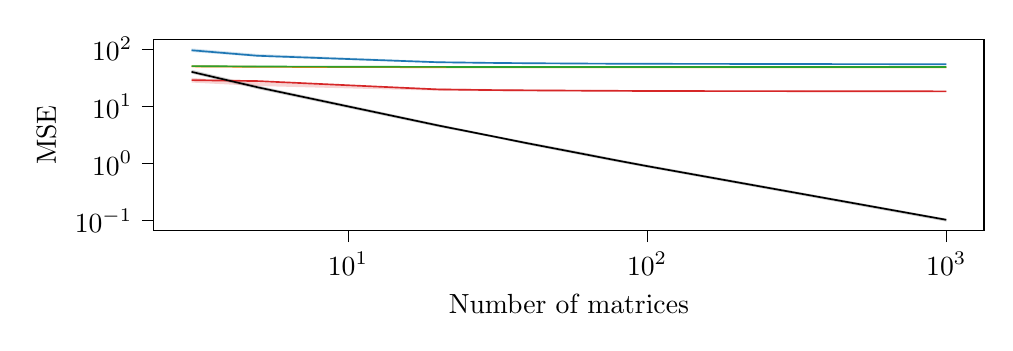
\begin{tikzpicture}

\definecolor{crimson2143940}{RGB}{214,39,40}
\definecolor{darkgray176}{RGB}{176,176,176}
\definecolor{darkorange25512714}{RGB}{255,127,14}
\definecolor{forestgreen4416044}{RGB}{44,160,44}
\definecolor{lightgray204}{RGB}{204,204,204}
\definecolor{steelblue31119180}{RGB}{31,119,180}

\begin{axis}[
width=\columnwidth,
height=4cm,
legend cell align={left},
legend style={
  fill opacity=0.8,
  draw opacity=1,
  text opacity=1,
  at={(0.03,0.03)},
  anchor=south west,
  draw=lightgray204
},
log basis x={10},
log basis y={10},
tick align=outside,
tick pos=left,
x grid style={darkgray176},
xlabel={Number of matrices},
xmin=2.2437647322819, xmax=1337.03857487278,
xmode=log,
xtick style={color=black},
xtick={0.1,1,10,100,1000,10000,100000},
xticklabels={
  \(\displaystyle {10^{-1}}\),
  \(\displaystyle {10^{0}}\),
  \(\displaystyle {10^{1}}\),
  \(\displaystyle {10^{2}}\),
  \(\displaystyle {10^{3}}\),
  \(\displaystyle {10^{4}}\),
  \(\displaystyle {10^{5}}\)
},
y grid style={darkgray176},
ylabel={MSE},
ymin=0.0676548185109966, ymax=144.054646180187,
ymode=log,
ytick style={color=black},
ytick={0.001,0.01,0.1,1,10,100,1000,10000},
yticklabels={
  \(\displaystyle {10^{-3}}\),
  \(\displaystyle {10^{-2}}\),
  \(\displaystyle {10^{-1}}\),
  \(\displaystyle {10^{0}}\),
  \(\displaystyle {10^{1}}\),
  \(\displaystyle {10^{2}}\),
  \(\displaystyle {10^{3}}\),
  \(\displaystyle {10^{4}}\)
}
]
\path [fill=steelblue31119180, fill opacity=0.2]
(axis cs:3,101.68201754882)
--(axis cs:3,88.1423662873149)
--(axis cs:5,72.3646618018412)
--(axis cs:20,56.3033594985253)
--(axis cs:30,55.2122414783319)
--(axis cs:40,54.4950492410911)
--(axis cs:60,54.3558372086263)
--(axis cs:80,53.9864569962276)
--(axis cs:100,53.7818808983528)
--(axis cs:1000,52.8842317120235)
--(axis cs:1000,54.1727833123211)
--(axis cs:1000,54.1727833123211)
--(axis cs:100,55.8890710915269)
--(axis cs:80,55.6871970646347)
--(axis cs:60,56.5784776906101)
--(axis cs:40,57.5926819637511)
--(axis cs:30,58.5444375596705)
--(axis cs:20,60.5980312773159)
--(axis cs:5,81.2598670477539)
--(axis cs:3,101.68201754882)
--cycle;

\path [fill=darkorange25512714, fill opacity=0.2]
(axis cs:3,50.9399401272127)
--(axis cs:3,47.616536256823)
--(axis cs:5,47.1612726433819)
--(axis cs:20,46.971955455793)
--(axis cs:30,47.0758081405333)
--(axis cs:40,47.0743333453457)
--(axis cs:60,46.9317172587414)
--(axis cs:80,47.0430248464519)
--(axis cs:100,47.0799238425103)
--(axis cs:1000,47.2703348549419)
--(axis cs:1000,47.4727762654529)
--(axis cs:1000,47.4727762654529)
--(axis cs:100,47.7556083668789)
--(axis cs:80,47.8016846942594)
--(axis cs:60,47.8594004527294)
--(axis cs:40,47.9763694452678)
--(axis cs:30,48.0504043908302)
--(axis cs:20,48.4899285925643)
--(axis cs:5,49.631305562104)
--(axis cs:3,50.9399401272127)
--cycle;

\path [fill=forestgreen4416044, fill opacity=0.2]
(axis cs:3,51.5543217681294)
--(axis cs:3,48.2174174363328)
--(axis cs:5,47.9435416290828)
--(axis cs:20,47.6022899376881)
--(axis cs:30,47.6905471249209)
--(axis cs:40,47.7473683750189)
--(axis cs:60,47.6137157519845)
--(axis cs:80,47.7378059813306)
--(axis cs:100,47.7700646928333)
--(axis cs:1000,47.947629843197)
--(axis cs:1000,48.1690500555604)
--(axis cs:1000,48.1690500555604)
--(axis cs:100,48.4186590813945)
--(axis cs:80,48.4745541082452)
--(axis cs:60,48.5534576983601)
--(axis cs:40,48.6446214322934)
--(axis cs:30,48.8034004170963)
--(axis cs:20,49.0483158707114)
--(axis cs:5,50.2587948881218)
--(axis cs:3,51.5543217681294)
--cycle;

\path [fill=crimson2143940, fill opacity=0.2]
(axis cs:3,31.0620901659341)
--(axis cs:3,25.7814354065144)
--(axis cs:5,22.4151766483135)
--(axis cs:20,18.5613287460143)
--(axis cs:30,18.2068668295756)
--(axis cs:40,18.0053951577646)
--(axis cs:60,18.0719911571276)
--(axis cs:80,18.0540496547627)
--(axis cs:100,17.8175733279627)
--(axis cs:1000,17.9286725829367)
--(axis cs:1000,18.2797926395433)
--(axis cs:1000,18.2797926395433)
--(axis cs:100,18.8026404764028)
--(axis cs:80,18.9858881503917)
--(axis cs:60,19.1340577061154)
--(axis cs:40,19.5820574055868)
--(axis cs:30,19.8302337288776)
--(axis cs:20,20.3582799108111)
--(axis cs:5,26.0822272030139)
--(axis cs:3,31.0620901659341)
--cycle;

\path [fill=black, fill opacity=0.2]
(axis cs:3,43.0134914235546)
--(axis cs:3,37.0492981565219)
--(axis cs:5,19.756909188043)
--(axis cs:20,4.31132775896778)
--(axis cs:30,2.86976889713881)
--(axis cs:40,2.09763141896607)
--(axis cs:60,1.39543284162807)
--(axis cs:80,1.04403044418553)
--(axis cs:100,0.842579436435285)
--(axis cs:1000,0.0958477337284056)
--(axis cs:1000,0.108031285268237)
--(axis cs:1000,0.108031285268237)
--(axis cs:100,0.944582470496131)
--(axis cs:80,1.17145085610537)
--(axis cs:60,1.5782483886311)
--(axis cs:40,2.3540862718306)
--(axis cs:30,3.154578637464)
--(axis cs:20,4.84674945358772)
--(axis cs:5,22.7658116599057)
--(axis cs:3,43.0134914235546)
--cycle;

\addplot [semithick, steelblue31119180]
table {%
3 94.5157592925942
5 75.6586882309294
20 58.353278559489
30 56.8241460264265
40 56.0826200766897
60 55.3597906632788
80 54.9424181564402
100 54.8161336747953
1000 53.7897210817627
};
\addlegendentry{SCM}
\addplot [semithick, darkorange25512714]
table {%
3 49.3613074737249
5 48.483748351865
20 47.6761402802835
30 47.5720824300155
40 47.5095728646513
60 47.4147988906565
80 47.4285959048943
100 47.4332061562883
1000 47.3704802116759
};
\addlegendentry{LW linear}
\addplot [semithick, forestgreen4416044]
table {%
3 49.9280772828501
5 49.1190938760236
20 48.3424993688959
30 48.2593143364372
40 48.1882416288635
60 48.097836189495
80 48.0973273595286
100 48.1184165931483
1000 48.0624897968217
};
\addlegendentry{OAS}
\addplot [semithick, crimson2143940]
table {%
3 28.4039460003532
5 27.3315303143067
20 19.5467182255244
30 19.0379044881684
40 18.8116447240747
60 18.5874615737571
80 18.4667134698607
100 18.3262967067618
1000 18.0866390671002
};
\addlegendentry{LW nonlinear}
\addplot [semithick, black]
table {%
3 39.6510294255462
5 21.2484674975276
20 4.58847604525462
30 3.01179037254277
40 2.22860231661461
60 1.48283062300453
80 1.1099362145875
100 0.892233532399277
1000 0.102898126015732
};
\addlegendentry{RMT}

\legend{};
\end{axis}

\end{tikzpicture}

    \caption{$p=5$, $n=7$}
    \label{fig:subfiga}
  \end{subfigure}
  \begin{subfigure}{0.4\textwidth}
    % This file was created with tikzplotlib v0.10.1.
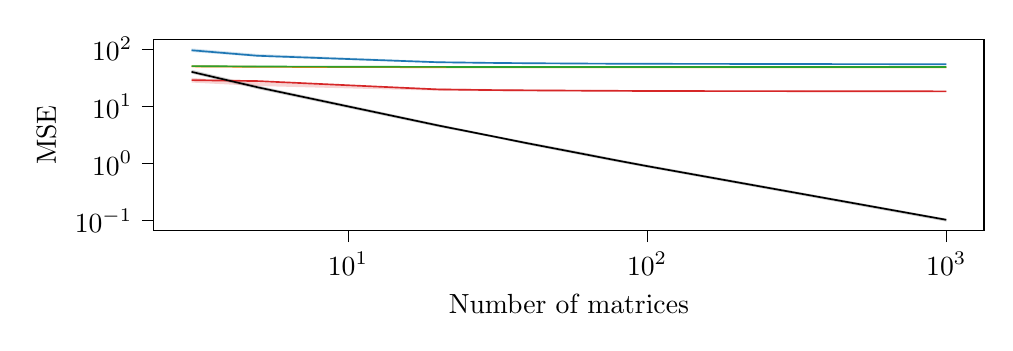
\begin{tikzpicture}

\definecolor{crimson2143940}{RGB}{214,39,40}
\definecolor{darkgray176}{RGB}{176,176,176}
\definecolor{darkorange25512714}{RGB}{255,127,14}
\definecolor{forestgreen4416044}{RGB}{44,160,44}
\definecolor{lightgray204}{RGB}{204,204,204}
\definecolor{steelblue31119180}{RGB}{31,119,180}

\begin{axis}[
width=\columnwidth,
height=4cm,
legend cell align={left},
legend style={
  fill opacity=0.8,
  draw opacity=1,
  text opacity=1,
  at={(0.03,0.03)},
  anchor=south west,
  draw=lightgray204
},
log basis x={10},
log basis y={10},
tick align=outside,
tick pos=left,
x grid style={darkgray176},
xlabel={Number of matrices},
xmin=2.2437647322819, xmax=1337.03857487278,
xmode=log,
xtick style={color=black},
xtick={0.1,1,10,100,1000,10000,100000},
xticklabels={
  \(\displaystyle {10^{-1}}\),
  \(\displaystyle {10^{0}}\),
  \(\displaystyle {10^{1}}\),
  \(\displaystyle {10^{2}}\),
  \(\displaystyle {10^{3}}\),
  \(\displaystyle {10^{4}}\),
  \(\displaystyle {10^{5}}\)
},
y grid style={darkgray176},
ylabel={MSE},
ymin=0.0676548185109966, ymax=144.054646180187,
ymode=log,
ytick style={color=black},
ytick={0.001,0.01,0.1,1,10,100,1000,10000},
yticklabels={
  \(\displaystyle {10^{-3}}\),
  \(\displaystyle {10^{-2}}\),
  \(\displaystyle {10^{-1}}\),
  \(\displaystyle {10^{0}}\),
  \(\displaystyle {10^{1}}\),
  \(\displaystyle {10^{2}}\),
  \(\displaystyle {10^{3}}\),
  \(\displaystyle {10^{4}}\)
}
]
\path [fill=steelblue31119180, fill opacity=0.2]
(axis cs:3,101.68201754882)
--(axis cs:3,88.1423662873149)
--(axis cs:5,72.3646618018412)
--(axis cs:20,56.3033594985253)
--(axis cs:30,55.2122414783319)
--(axis cs:40,54.4950492410911)
--(axis cs:60,54.3558372086263)
--(axis cs:80,53.9864569962276)
--(axis cs:100,53.7818808983528)
--(axis cs:1000,52.8842317120235)
--(axis cs:1000,54.1727833123211)
--(axis cs:1000,54.1727833123211)
--(axis cs:100,55.8890710915269)
--(axis cs:80,55.6871970646347)
--(axis cs:60,56.5784776906101)
--(axis cs:40,57.5926819637511)
--(axis cs:30,58.5444375596705)
--(axis cs:20,60.5980312773159)
--(axis cs:5,81.2598670477539)
--(axis cs:3,101.68201754882)
--cycle;

\path [fill=darkorange25512714, fill opacity=0.2]
(axis cs:3,50.9399401272127)
--(axis cs:3,47.616536256823)
--(axis cs:5,47.1612726433819)
--(axis cs:20,46.971955455793)
--(axis cs:30,47.0758081405333)
--(axis cs:40,47.0743333453457)
--(axis cs:60,46.9317172587414)
--(axis cs:80,47.0430248464519)
--(axis cs:100,47.0799238425103)
--(axis cs:1000,47.2703348549419)
--(axis cs:1000,47.4727762654529)
--(axis cs:1000,47.4727762654529)
--(axis cs:100,47.7556083668789)
--(axis cs:80,47.8016846942594)
--(axis cs:60,47.8594004527294)
--(axis cs:40,47.9763694452678)
--(axis cs:30,48.0504043908302)
--(axis cs:20,48.4899285925643)
--(axis cs:5,49.631305562104)
--(axis cs:3,50.9399401272127)
--cycle;

\path [fill=forestgreen4416044, fill opacity=0.2]
(axis cs:3,51.5543217681294)
--(axis cs:3,48.2174174363328)
--(axis cs:5,47.9435416290828)
--(axis cs:20,47.6022899376881)
--(axis cs:30,47.6905471249209)
--(axis cs:40,47.7473683750189)
--(axis cs:60,47.6137157519845)
--(axis cs:80,47.7378059813306)
--(axis cs:100,47.7700646928333)
--(axis cs:1000,47.947629843197)
--(axis cs:1000,48.1690500555604)
--(axis cs:1000,48.1690500555604)
--(axis cs:100,48.4186590813945)
--(axis cs:80,48.4745541082452)
--(axis cs:60,48.5534576983601)
--(axis cs:40,48.6446214322934)
--(axis cs:30,48.8034004170963)
--(axis cs:20,49.0483158707114)
--(axis cs:5,50.2587948881218)
--(axis cs:3,51.5543217681294)
--cycle;

\path [fill=crimson2143940, fill opacity=0.2]
(axis cs:3,31.0620901659341)
--(axis cs:3,25.7814354065144)
--(axis cs:5,22.4151766483135)
--(axis cs:20,18.5613287460143)
--(axis cs:30,18.2068668295756)
--(axis cs:40,18.0053951577646)
--(axis cs:60,18.0719911571276)
--(axis cs:80,18.0540496547627)
--(axis cs:100,17.8175733279627)
--(axis cs:1000,17.9286725829367)
--(axis cs:1000,18.2797926395433)
--(axis cs:1000,18.2797926395433)
--(axis cs:100,18.8026404764028)
--(axis cs:80,18.9858881503917)
--(axis cs:60,19.1340577061154)
--(axis cs:40,19.5820574055868)
--(axis cs:30,19.8302337288776)
--(axis cs:20,20.3582799108111)
--(axis cs:5,26.0822272030139)
--(axis cs:3,31.0620901659341)
--cycle;

\path [fill=black, fill opacity=0.2]
(axis cs:3,43.0134914235546)
--(axis cs:3,37.0492981565219)
--(axis cs:5,19.756909188043)
--(axis cs:20,4.31132775896778)
--(axis cs:30,2.86976889713881)
--(axis cs:40,2.09763141896607)
--(axis cs:60,1.39543284162807)
--(axis cs:80,1.04403044418553)
--(axis cs:100,0.842579436435285)
--(axis cs:1000,0.0958477337284056)
--(axis cs:1000,0.108031285268237)
--(axis cs:1000,0.108031285268237)
--(axis cs:100,0.944582470496131)
--(axis cs:80,1.17145085610537)
--(axis cs:60,1.5782483886311)
--(axis cs:40,2.3540862718306)
--(axis cs:30,3.154578637464)
--(axis cs:20,4.84674945358772)
--(axis cs:5,22.7658116599057)
--(axis cs:3,43.0134914235546)
--cycle;

\addplot [semithick, steelblue31119180]
table {%
3 94.5157592925942
5 75.6586882309294
20 58.353278559489
30 56.8241460264265
40 56.0826200766897
60 55.3597906632788
80 54.9424181564402
100 54.8161336747953
1000 53.7897210817627
};
\addlegendentry{SCM}
\addplot [semithick, darkorange25512714]
table {%
3 49.3613074737249
5 48.483748351865
20 47.6761402802835
30 47.5720824300155
40 47.5095728646513
60 47.4147988906565
80 47.4285959048943
100 47.4332061562883
1000 47.3704802116759
};
\addlegendentry{LW linear}
\addplot [semithick, forestgreen4416044]
table {%
3 49.9280772828501
5 49.1190938760236
20 48.3424993688959
30 48.2593143364372
40 48.1882416288635
60 48.097836189495
80 48.0973273595286
100 48.1184165931483
1000 48.0624897968217
};
\addlegendentry{OAS}
\addplot [semithick, crimson2143940]
table {%
3 28.4039460003532
5 27.3315303143067
20 19.5467182255244
30 19.0379044881684
40 18.8116447240747
60 18.5874615737571
80 18.4667134698607
100 18.3262967067618
1000 18.0866390671002
};
\addlegendentry{LW nonlinear}
\addplot [semithick, black]
table {%
3 39.6510294255462
5 21.2484674975276
20 4.58847604525462
30 3.01179037254277
40 2.22860231661461
60 1.48283062300453
80 1.1099362145875
100 0.892233532399277
1000 0.102898126015732
};
\addlegendentry{RMT}

\legend{};
\end{axis}

\end{tikzpicture}

    \caption{$p=5$, $n=25$}
    \label{fig:subfigb}
  \end{subfigure}
  \begin{subfigure}{0.4\textwidth}
    % This file was created with tikzplotlib v0.10.1.
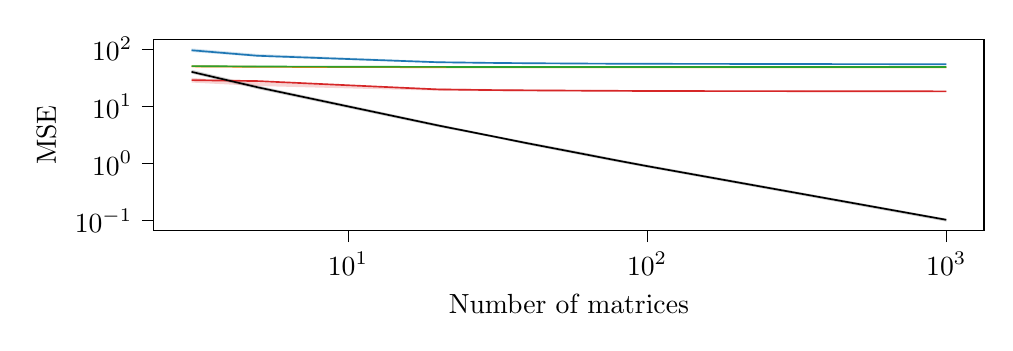
\begin{tikzpicture}

\definecolor{crimson2143940}{RGB}{214,39,40}
\definecolor{darkgray176}{RGB}{176,176,176}
\definecolor{darkorange25512714}{RGB}{255,127,14}
\definecolor{forestgreen4416044}{RGB}{44,160,44}
\definecolor{lightgray204}{RGB}{204,204,204}
\definecolor{steelblue31119180}{RGB}{31,119,180}

\begin{axis}[
width=\columnwidth,
height=4cm,
legend cell align={left},
legend style={
  fill opacity=0.8,
  draw opacity=1,
  text opacity=1,
  at={(0.03,0.03)},
  anchor=south west,
  draw=lightgray204
},
log basis x={10},
log basis y={10},
tick align=outside,
tick pos=left,
x grid style={darkgray176},
xlabel={Number of matrices},
xmin=2.2437647322819, xmax=1337.03857487278,
xmode=log,
xtick style={color=black},
xtick={0.1,1,10,100,1000,10000,100000},
xticklabels={
  \(\displaystyle {10^{-1}}\),
  \(\displaystyle {10^{0}}\),
  \(\displaystyle {10^{1}}\),
  \(\displaystyle {10^{2}}\),
  \(\displaystyle {10^{3}}\),
  \(\displaystyle {10^{4}}\),
  \(\displaystyle {10^{5}}\)
},
y grid style={darkgray176},
ylabel={MSE},
ymin=0.0676548185109966, ymax=144.054646180187,
ymode=log,
ytick style={color=black},
ytick={0.001,0.01,0.1,1,10,100,1000,10000},
yticklabels={
  \(\displaystyle {10^{-3}}\),
  \(\displaystyle {10^{-2}}\),
  \(\displaystyle {10^{-1}}\),
  \(\displaystyle {10^{0}}\),
  \(\displaystyle {10^{1}}\),
  \(\displaystyle {10^{2}}\),
  \(\displaystyle {10^{3}}\),
  \(\displaystyle {10^{4}}\)
}
]
\path [fill=steelblue31119180, fill opacity=0.2]
(axis cs:3,101.68201754882)
--(axis cs:3,88.1423662873149)
--(axis cs:5,72.3646618018412)
--(axis cs:20,56.3033594985253)
--(axis cs:30,55.2122414783319)
--(axis cs:40,54.4950492410911)
--(axis cs:60,54.3558372086263)
--(axis cs:80,53.9864569962276)
--(axis cs:100,53.7818808983528)
--(axis cs:1000,52.8842317120235)
--(axis cs:1000,54.1727833123211)
--(axis cs:1000,54.1727833123211)
--(axis cs:100,55.8890710915269)
--(axis cs:80,55.6871970646347)
--(axis cs:60,56.5784776906101)
--(axis cs:40,57.5926819637511)
--(axis cs:30,58.5444375596705)
--(axis cs:20,60.5980312773159)
--(axis cs:5,81.2598670477539)
--(axis cs:3,101.68201754882)
--cycle;

\path [fill=darkorange25512714, fill opacity=0.2]
(axis cs:3,50.9399401272127)
--(axis cs:3,47.616536256823)
--(axis cs:5,47.1612726433819)
--(axis cs:20,46.971955455793)
--(axis cs:30,47.0758081405333)
--(axis cs:40,47.0743333453457)
--(axis cs:60,46.9317172587414)
--(axis cs:80,47.0430248464519)
--(axis cs:100,47.0799238425103)
--(axis cs:1000,47.2703348549419)
--(axis cs:1000,47.4727762654529)
--(axis cs:1000,47.4727762654529)
--(axis cs:100,47.7556083668789)
--(axis cs:80,47.8016846942594)
--(axis cs:60,47.8594004527294)
--(axis cs:40,47.9763694452678)
--(axis cs:30,48.0504043908302)
--(axis cs:20,48.4899285925643)
--(axis cs:5,49.631305562104)
--(axis cs:3,50.9399401272127)
--cycle;

\path [fill=forestgreen4416044, fill opacity=0.2]
(axis cs:3,51.5543217681294)
--(axis cs:3,48.2174174363328)
--(axis cs:5,47.9435416290828)
--(axis cs:20,47.6022899376881)
--(axis cs:30,47.6905471249209)
--(axis cs:40,47.7473683750189)
--(axis cs:60,47.6137157519845)
--(axis cs:80,47.7378059813306)
--(axis cs:100,47.7700646928333)
--(axis cs:1000,47.947629843197)
--(axis cs:1000,48.1690500555604)
--(axis cs:1000,48.1690500555604)
--(axis cs:100,48.4186590813945)
--(axis cs:80,48.4745541082452)
--(axis cs:60,48.5534576983601)
--(axis cs:40,48.6446214322934)
--(axis cs:30,48.8034004170963)
--(axis cs:20,49.0483158707114)
--(axis cs:5,50.2587948881218)
--(axis cs:3,51.5543217681294)
--cycle;

\path [fill=crimson2143940, fill opacity=0.2]
(axis cs:3,31.0620901659341)
--(axis cs:3,25.7814354065144)
--(axis cs:5,22.4151766483135)
--(axis cs:20,18.5613287460143)
--(axis cs:30,18.2068668295756)
--(axis cs:40,18.0053951577646)
--(axis cs:60,18.0719911571276)
--(axis cs:80,18.0540496547627)
--(axis cs:100,17.8175733279627)
--(axis cs:1000,17.9286725829367)
--(axis cs:1000,18.2797926395433)
--(axis cs:1000,18.2797926395433)
--(axis cs:100,18.8026404764028)
--(axis cs:80,18.9858881503917)
--(axis cs:60,19.1340577061154)
--(axis cs:40,19.5820574055868)
--(axis cs:30,19.8302337288776)
--(axis cs:20,20.3582799108111)
--(axis cs:5,26.0822272030139)
--(axis cs:3,31.0620901659341)
--cycle;

\path [fill=black, fill opacity=0.2]
(axis cs:3,43.0134914235546)
--(axis cs:3,37.0492981565219)
--(axis cs:5,19.756909188043)
--(axis cs:20,4.31132775896778)
--(axis cs:30,2.86976889713881)
--(axis cs:40,2.09763141896607)
--(axis cs:60,1.39543284162807)
--(axis cs:80,1.04403044418553)
--(axis cs:100,0.842579436435285)
--(axis cs:1000,0.0958477337284056)
--(axis cs:1000,0.108031285268237)
--(axis cs:1000,0.108031285268237)
--(axis cs:100,0.944582470496131)
--(axis cs:80,1.17145085610537)
--(axis cs:60,1.5782483886311)
--(axis cs:40,2.3540862718306)
--(axis cs:30,3.154578637464)
--(axis cs:20,4.84674945358772)
--(axis cs:5,22.7658116599057)
--(axis cs:3,43.0134914235546)
--cycle;

\addplot [semithick, steelblue31119180]
table {%
3 94.5157592925942
5 75.6586882309294
20 58.353278559489
30 56.8241460264265
40 56.0826200766897
60 55.3597906632788
80 54.9424181564402
100 54.8161336747953
1000 53.7897210817627
};
\addlegendentry{SCM}
\addplot [semithick, darkorange25512714]
table {%
3 49.3613074737249
5 48.483748351865
20 47.6761402802835
30 47.5720824300155
40 47.5095728646513
60 47.4147988906565
80 47.4285959048943
100 47.4332061562883
1000 47.3704802116759
};
\addlegendentry{LW linear}
\addplot [semithick, forestgreen4416044]
table {%
3 49.9280772828501
5 49.1190938760236
20 48.3424993688959
30 48.2593143364372
40 48.1882416288635
60 48.097836189495
80 48.0973273595286
100 48.1184165931483
1000 48.0624897968217
};
\addlegendentry{OAS}
\addplot [semithick, crimson2143940]
table {%
3 28.4039460003532
5 27.3315303143067
20 19.5467182255244
30 19.0379044881684
40 18.8116447240747
60 18.5874615737571
80 18.4667134698607
100 18.3262967067618
1000 18.0866390671002
};
\addlegendentry{LW nonlinear}
\addplot [semithick, black]
table {%
3 39.6510294255462
5 21.2484674975276
20 4.58847604525462
30 3.01179037254277
40 2.22860231661461
60 1.48283062300453
80 1.1099362145875
100 0.892233532399277
1000 0.102898126015732
};
\addlegendentry{RMT}

\legend{};
\end{axis}

\end{tikzpicture}

    \caption{$p=64$, $n=66$}
    \label{fig:subfiga}
  \end{subfigure}
  \begin{subfigure}{0.4\textwidth}
    % This file was created with tikzplotlib v0.10.1.
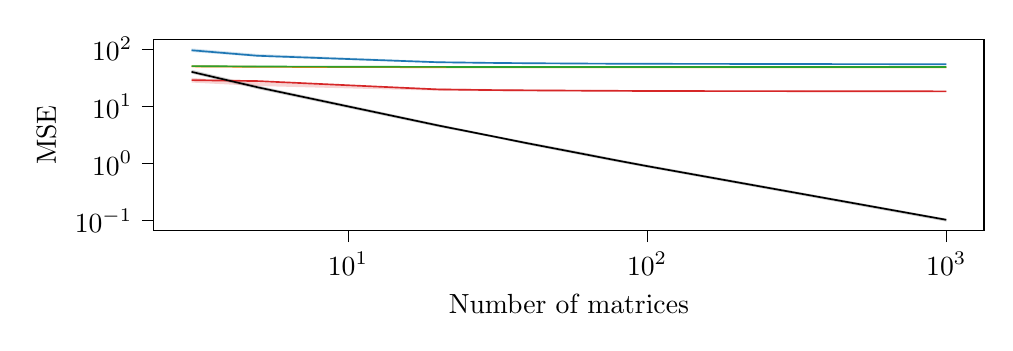
\begin{tikzpicture}

\definecolor{crimson2143940}{RGB}{214,39,40}
\definecolor{darkgray176}{RGB}{176,176,176}
\definecolor{darkorange25512714}{RGB}{255,127,14}
\definecolor{forestgreen4416044}{RGB}{44,160,44}
\definecolor{lightgray204}{RGB}{204,204,204}
\definecolor{steelblue31119180}{RGB}{31,119,180}

\begin{axis}[
width=\columnwidth,
height=4cm,
legend cell align={left},
legend style={
  fill opacity=0.8,
  draw opacity=1,
  text opacity=1,
  at={(0.03,0.03)},
  anchor=south west,
  draw=lightgray204
},
log basis x={10},
log basis y={10},
tick align=outside,
tick pos=left,
x grid style={darkgray176},
xlabel={Number of matrices},
xmin=2.2437647322819, xmax=1337.03857487278,
xmode=log,
xtick style={color=black},
xtick={0.1,1,10,100,1000,10000,100000},
xticklabels={
  \(\displaystyle {10^{-1}}\),
  \(\displaystyle {10^{0}}\),
  \(\displaystyle {10^{1}}\),
  \(\displaystyle {10^{2}}\),
  \(\displaystyle {10^{3}}\),
  \(\displaystyle {10^{4}}\),
  \(\displaystyle {10^{5}}\)
},
y grid style={darkgray176},
ylabel={MSE},
ymin=0.0676548185109966, ymax=144.054646180187,
ymode=log,
ytick style={color=black},
ytick={0.001,0.01,0.1,1,10,100,1000,10000},
yticklabels={
  \(\displaystyle {10^{-3}}\),
  \(\displaystyle {10^{-2}}\),
  \(\displaystyle {10^{-1}}\),
  \(\displaystyle {10^{0}}\),
  \(\displaystyle {10^{1}}\),
  \(\displaystyle {10^{2}}\),
  \(\displaystyle {10^{3}}\),
  \(\displaystyle {10^{4}}\)
}
]
\path [fill=steelblue31119180, fill opacity=0.2]
(axis cs:3,101.68201754882)
--(axis cs:3,88.1423662873149)
--(axis cs:5,72.3646618018412)
--(axis cs:20,56.3033594985253)
--(axis cs:30,55.2122414783319)
--(axis cs:40,54.4950492410911)
--(axis cs:60,54.3558372086263)
--(axis cs:80,53.9864569962276)
--(axis cs:100,53.7818808983528)
--(axis cs:1000,52.8842317120235)
--(axis cs:1000,54.1727833123211)
--(axis cs:1000,54.1727833123211)
--(axis cs:100,55.8890710915269)
--(axis cs:80,55.6871970646347)
--(axis cs:60,56.5784776906101)
--(axis cs:40,57.5926819637511)
--(axis cs:30,58.5444375596705)
--(axis cs:20,60.5980312773159)
--(axis cs:5,81.2598670477539)
--(axis cs:3,101.68201754882)
--cycle;

\path [fill=darkorange25512714, fill opacity=0.2]
(axis cs:3,50.9399401272127)
--(axis cs:3,47.616536256823)
--(axis cs:5,47.1612726433819)
--(axis cs:20,46.971955455793)
--(axis cs:30,47.0758081405333)
--(axis cs:40,47.0743333453457)
--(axis cs:60,46.9317172587414)
--(axis cs:80,47.0430248464519)
--(axis cs:100,47.0799238425103)
--(axis cs:1000,47.2703348549419)
--(axis cs:1000,47.4727762654529)
--(axis cs:1000,47.4727762654529)
--(axis cs:100,47.7556083668789)
--(axis cs:80,47.8016846942594)
--(axis cs:60,47.8594004527294)
--(axis cs:40,47.9763694452678)
--(axis cs:30,48.0504043908302)
--(axis cs:20,48.4899285925643)
--(axis cs:5,49.631305562104)
--(axis cs:3,50.9399401272127)
--cycle;

\path [fill=forestgreen4416044, fill opacity=0.2]
(axis cs:3,51.5543217681294)
--(axis cs:3,48.2174174363328)
--(axis cs:5,47.9435416290828)
--(axis cs:20,47.6022899376881)
--(axis cs:30,47.6905471249209)
--(axis cs:40,47.7473683750189)
--(axis cs:60,47.6137157519845)
--(axis cs:80,47.7378059813306)
--(axis cs:100,47.7700646928333)
--(axis cs:1000,47.947629843197)
--(axis cs:1000,48.1690500555604)
--(axis cs:1000,48.1690500555604)
--(axis cs:100,48.4186590813945)
--(axis cs:80,48.4745541082452)
--(axis cs:60,48.5534576983601)
--(axis cs:40,48.6446214322934)
--(axis cs:30,48.8034004170963)
--(axis cs:20,49.0483158707114)
--(axis cs:5,50.2587948881218)
--(axis cs:3,51.5543217681294)
--cycle;

\path [fill=crimson2143940, fill opacity=0.2]
(axis cs:3,31.0620901659341)
--(axis cs:3,25.7814354065144)
--(axis cs:5,22.4151766483135)
--(axis cs:20,18.5613287460143)
--(axis cs:30,18.2068668295756)
--(axis cs:40,18.0053951577646)
--(axis cs:60,18.0719911571276)
--(axis cs:80,18.0540496547627)
--(axis cs:100,17.8175733279627)
--(axis cs:1000,17.9286725829367)
--(axis cs:1000,18.2797926395433)
--(axis cs:1000,18.2797926395433)
--(axis cs:100,18.8026404764028)
--(axis cs:80,18.9858881503917)
--(axis cs:60,19.1340577061154)
--(axis cs:40,19.5820574055868)
--(axis cs:30,19.8302337288776)
--(axis cs:20,20.3582799108111)
--(axis cs:5,26.0822272030139)
--(axis cs:3,31.0620901659341)
--cycle;

\path [fill=black, fill opacity=0.2]
(axis cs:3,43.0134914235546)
--(axis cs:3,37.0492981565219)
--(axis cs:5,19.756909188043)
--(axis cs:20,4.31132775896778)
--(axis cs:30,2.86976889713881)
--(axis cs:40,2.09763141896607)
--(axis cs:60,1.39543284162807)
--(axis cs:80,1.04403044418553)
--(axis cs:100,0.842579436435285)
--(axis cs:1000,0.0958477337284056)
--(axis cs:1000,0.108031285268237)
--(axis cs:1000,0.108031285268237)
--(axis cs:100,0.944582470496131)
--(axis cs:80,1.17145085610537)
--(axis cs:60,1.5782483886311)
--(axis cs:40,2.3540862718306)
--(axis cs:30,3.154578637464)
--(axis cs:20,4.84674945358772)
--(axis cs:5,22.7658116599057)
--(axis cs:3,43.0134914235546)
--cycle;

\addplot [semithick, steelblue31119180]
table {%
3 94.5157592925942
5 75.6586882309294
20 58.353278559489
30 56.8241460264265
40 56.0826200766897
60 55.3597906632788
80 54.9424181564402
100 54.8161336747953
1000 53.7897210817627
};
\addlegendentry{SCM}
\addplot [semithick, darkorange25512714]
table {%
3 49.3613074737249
5 48.483748351865
20 47.6761402802835
30 47.5720824300155
40 47.5095728646513
60 47.4147988906565
80 47.4285959048943
100 47.4332061562883
1000 47.3704802116759
};
\addlegendentry{LW linear}
\addplot [semithick, forestgreen4416044]
table {%
3 49.9280772828501
5 49.1190938760236
20 48.3424993688959
30 48.2593143364372
40 48.1882416288635
60 48.097836189495
80 48.0973273595286
100 48.1184165931483
1000 48.0624897968217
};
\addlegendentry{OAS}
\addplot [semithick, crimson2143940]
table {%
3 28.4039460003532
5 27.3315303143067
20 19.5467182255244
30 19.0379044881684
40 18.8116447240747
60 18.5874615737571
80 18.4667134698607
100 18.3262967067618
1000 18.0866390671002
};
\addlegendentry{LW nonlinear}
\addplot [semithick, black]
table {%
3 39.6510294255462
5 21.2484674975276
20 4.58847604525462
30 3.01179037254277
40 2.22860231661461
60 1.48283062300453
80 1.1099362145875
100 0.892233532399277
1000 0.102898126015732
};
\addlegendentry{RMT}

\legend{};
\end{axis}

\end{tikzpicture}

    \caption{$p=64$, $n=128$}
    \label{fig:subfigb}
  \end{subfigure}
  \begin{subfigure}{0.4\textwidth}
    % This file was created with tikzplotlib v0.10.1.
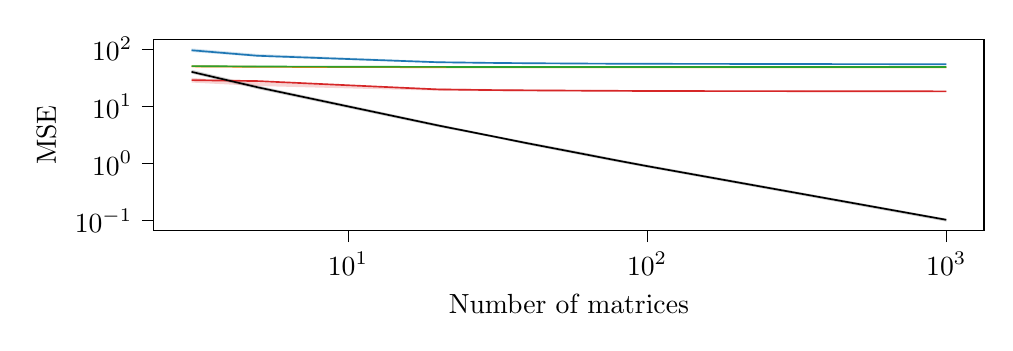
\begin{tikzpicture}

\definecolor{crimson2143940}{RGB}{214,39,40}
\definecolor{darkgray176}{RGB}{176,176,176}
\definecolor{darkorange25512714}{RGB}{255,127,14}
\definecolor{forestgreen4416044}{RGB}{44,160,44}
\definecolor{lightgray204}{RGB}{204,204,204}
\definecolor{steelblue31119180}{RGB}{31,119,180}

\begin{axis}[
width=\columnwidth,
height=4cm,
legend cell align={left},
legend style={
  fill opacity=0.8,
  draw opacity=1,
  text opacity=1,
  at={(0.03,0.03)},
  anchor=south west,
  draw=lightgray204
},
log basis x={10},
log basis y={10},
tick align=outside,
tick pos=left,
x grid style={darkgray176},
xlabel={Number of matrices},
xmin=2.2437647322819, xmax=1337.03857487278,
xmode=log,
xtick style={color=black},
xtick={0.1,1,10,100,1000,10000,100000},
xticklabels={
  \(\displaystyle {10^{-1}}\),
  \(\displaystyle {10^{0}}\),
  \(\displaystyle {10^{1}}\),
  \(\displaystyle {10^{2}}\),
  \(\displaystyle {10^{3}}\),
  \(\displaystyle {10^{4}}\),
  \(\displaystyle {10^{5}}\)
},
y grid style={darkgray176},
ylabel={MSE},
ymin=0.0676548185109966, ymax=144.054646180187,
ymode=log,
ytick style={color=black},
ytick={0.001,0.01,0.1,1,10,100,1000,10000},
yticklabels={
  \(\displaystyle {10^{-3}}\),
  \(\displaystyle {10^{-2}}\),
  \(\displaystyle {10^{-1}}\),
  \(\displaystyle {10^{0}}\),
  \(\displaystyle {10^{1}}\),
  \(\displaystyle {10^{2}}\),
  \(\displaystyle {10^{3}}\),
  \(\displaystyle {10^{4}}\)
}
]
\path [fill=steelblue31119180, fill opacity=0.2]
(axis cs:3,101.68201754882)
--(axis cs:3,88.1423662873149)
--(axis cs:5,72.3646618018412)
--(axis cs:20,56.3033594985253)
--(axis cs:30,55.2122414783319)
--(axis cs:40,54.4950492410911)
--(axis cs:60,54.3558372086263)
--(axis cs:80,53.9864569962276)
--(axis cs:100,53.7818808983528)
--(axis cs:1000,52.8842317120235)
--(axis cs:1000,54.1727833123211)
--(axis cs:1000,54.1727833123211)
--(axis cs:100,55.8890710915269)
--(axis cs:80,55.6871970646347)
--(axis cs:60,56.5784776906101)
--(axis cs:40,57.5926819637511)
--(axis cs:30,58.5444375596705)
--(axis cs:20,60.5980312773159)
--(axis cs:5,81.2598670477539)
--(axis cs:3,101.68201754882)
--cycle;

\path [fill=darkorange25512714, fill opacity=0.2]
(axis cs:3,50.9399401272127)
--(axis cs:3,47.616536256823)
--(axis cs:5,47.1612726433819)
--(axis cs:20,46.971955455793)
--(axis cs:30,47.0758081405333)
--(axis cs:40,47.0743333453457)
--(axis cs:60,46.9317172587414)
--(axis cs:80,47.0430248464519)
--(axis cs:100,47.0799238425103)
--(axis cs:1000,47.2703348549419)
--(axis cs:1000,47.4727762654529)
--(axis cs:1000,47.4727762654529)
--(axis cs:100,47.7556083668789)
--(axis cs:80,47.8016846942594)
--(axis cs:60,47.8594004527294)
--(axis cs:40,47.9763694452678)
--(axis cs:30,48.0504043908302)
--(axis cs:20,48.4899285925643)
--(axis cs:5,49.631305562104)
--(axis cs:3,50.9399401272127)
--cycle;

\path [fill=forestgreen4416044, fill opacity=0.2]
(axis cs:3,51.5543217681294)
--(axis cs:3,48.2174174363328)
--(axis cs:5,47.9435416290828)
--(axis cs:20,47.6022899376881)
--(axis cs:30,47.6905471249209)
--(axis cs:40,47.7473683750189)
--(axis cs:60,47.6137157519845)
--(axis cs:80,47.7378059813306)
--(axis cs:100,47.7700646928333)
--(axis cs:1000,47.947629843197)
--(axis cs:1000,48.1690500555604)
--(axis cs:1000,48.1690500555604)
--(axis cs:100,48.4186590813945)
--(axis cs:80,48.4745541082452)
--(axis cs:60,48.5534576983601)
--(axis cs:40,48.6446214322934)
--(axis cs:30,48.8034004170963)
--(axis cs:20,49.0483158707114)
--(axis cs:5,50.2587948881218)
--(axis cs:3,51.5543217681294)
--cycle;

\path [fill=crimson2143940, fill opacity=0.2]
(axis cs:3,31.0620901659341)
--(axis cs:3,25.7814354065144)
--(axis cs:5,22.4151766483135)
--(axis cs:20,18.5613287460143)
--(axis cs:30,18.2068668295756)
--(axis cs:40,18.0053951577646)
--(axis cs:60,18.0719911571276)
--(axis cs:80,18.0540496547627)
--(axis cs:100,17.8175733279627)
--(axis cs:1000,17.9286725829367)
--(axis cs:1000,18.2797926395433)
--(axis cs:1000,18.2797926395433)
--(axis cs:100,18.8026404764028)
--(axis cs:80,18.9858881503917)
--(axis cs:60,19.1340577061154)
--(axis cs:40,19.5820574055868)
--(axis cs:30,19.8302337288776)
--(axis cs:20,20.3582799108111)
--(axis cs:5,26.0822272030139)
--(axis cs:3,31.0620901659341)
--cycle;

\path [fill=black, fill opacity=0.2]
(axis cs:3,43.0134914235546)
--(axis cs:3,37.0492981565219)
--(axis cs:5,19.756909188043)
--(axis cs:20,4.31132775896778)
--(axis cs:30,2.86976889713881)
--(axis cs:40,2.09763141896607)
--(axis cs:60,1.39543284162807)
--(axis cs:80,1.04403044418553)
--(axis cs:100,0.842579436435285)
--(axis cs:1000,0.0958477337284056)
--(axis cs:1000,0.108031285268237)
--(axis cs:1000,0.108031285268237)
--(axis cs:100,0.944582470496131)
--(axis cs:80,1.17145085610537)
--(axis cs:60,1.5782483886311)
--(axis cs:40,2.3540862718306)
--(axis cs:30,3.154578637464)
--(axis cs:20,4.84674945358772)
--(axis cs:5,22.7658116599057)
--(axis cs:3,43.0134914235546)
--cycle;

\addplot [semithick, steelblue31119180]
table {%
3 94.5157592925942
5 75.6586882309294
20 58.353278559489
30 56.8241460264265
40 56.0826200766897
60 55.3597906632788
80 54.9424181564402
100 54.8161336747953
1000 53.7897210817627
};
\addlegendentry{SCM}
\addplot [semithick, darkorange25512714]
table {%
3 49.3613074737249
5 48.483748351865
20 47.6761402802835
30 47.5720824300155
40 47.5095728646513
60 47.4147988906565
80 47.4285959048943
100 47.4332061562883
1000 47.3704802116759
};
\addlegendentry{LW linear}
\addplot [semithick, forestgreen4416044]
table {%
3 49.9280772828501
5 49.1190938760236
20 48.3424993688959
30 48.2593143364372
40 48.1882416288635
60 48.097836189495
80 48.0973273595286
100 48.1184165931483
1000 48.0624897968217
};
\addlegendentry{OAS}
\addplot [semithick, crimson2143940]
table {%
3 28.4039460003532
5 27.3315303143067
20 19.5467182255244
30 19.0379044881684
40 18.8116447240747
60 18.5874615737571
80 18.4667134698607
100 18.3262967067618
1000 18.0866390671002
};
\addlegendentry{LW nonlinear}
\addplot [semithick, black]
table {%
3 39.6510294255462
5 21.2484674975276
20 4.58847604525462
30 3.01179037254277
40 2.22860231661461
60 1.48283062300453
80 1.1099362145875
100 0.892233532399277
1000 0.102898126015732
};
\addlegendentry{RMT}

\legend{};
\end{axis}

\end{tikzpicture}

    \caption{$p=64$, $n=512$}
    \label{fig:subfigb}
  \end{subfigure}
  
  \caption{MSE of the estimated mean towards true mean for different regimes. }
  \label{fig:mainfig}
\end{figure*}

\section{Test on real data}

\begin{table*}[]
    \centering
    \begin{tabular}{||c||c|c|c|c||}
    \hline
    \multicolumn{5}{|c|}{PhysionetMI, $p=64$, $K=5$, 23 trials/classes, 109 subjects} \\
    \hline
    Paradigm & SCM & LW-SCM & Non Linear LW & RMT-KM \\
    \hline
    [1,3], 80Hz & {\bf 0.493} & 0.397 & $\times$ & 0.49 \\
    \hline
    \hline
    \multicolumn{5}{|c|}{Schirrmeister2017, $p=128$, $K=4$, 120 trials/classes, 14 subjects} \\
    \hline
    Paradigm     & SCM         & LW-SCM & Non Linear LW & RMT-KM \\
    \hline
    [0,5], 100Hz & 0.597       & 0.483 & 0.561          & {\bf 0.603} \\
    \hline
    \hline
    \multicolumn{5}{|c|}{Cho2017, $p=64$, $K=2$, 100 trials/classes, 53 subjects} \\
    \hline
    Paradigm & SCM & LW-SCM & Non Linear LW & RMT-KM \\
    \hline
    [1,3], 128Hz & 0.615 & 0.609 & 0.601 & {\bf 0.622} \\
    \hline
    \hline
    \multicolumn{5}{|c|}{Lee2019, $p=62$, $K=2$, 100 trials/classes, 55 subjects} \\
    \hline
    Paradigm & SCM & LW-SCM & Non Linear LW & RMT-KM \\
    \hline
    [2,3], 100Hz & {\bf 0.666} & 0.642 & 0.626 & 0.66 \\
    \hline
    \hline
    \multicolumn{5}{|c|}{Weibo2014, $p=60$, $K=7$, 80 trials/classes, 10 subjects} \\
    \hline
    Paradigm & SCM & LW-SCM & Non Linear LW & RMT-KM \\
    \hline
    [1,3], 100Hz & {\bf 0.409} & 0.349 & $\times$ & 0.403 \\
    \hline
    \hline
    \multicolumn{5}{|c|}{MunichMI, $p=128$, $K=2$, 150 trials/classes, 10 subjects} \\
    \hline
    Paradigm & SCM & LW-SCM & Non Linear LW & RMT-KM \\
    \hline
    [0,7], 100Hz & 0.632 & 0.624 & $\times$ & {\bf 0.638} \\
    \hline
    \end{tabular}
    \caption{Classification results for motor imaging data}
    \label{tab:my_label}
\end{table*}




\begin{table*}[t]
\centering
\begin{tabular}{rcccccccc}
                              &               &                       & \multicolumn{2}{c}{SCM} & \multicolumn{2}{c}{LW-SCM} & \multicolumn{2}{c}{RMT}         \\
                              & data size $p$ & number of samples $n$ & acc             & mIoU  & acc          & mIoU        & acc            & mIoU           \\ \cline{2-9} 
\multirow{4}{*}{Indian pines} & 5             & 5$\times$5            & 0.385           & 0.278 & 0.302        & 0.204       & \textbf{0.454} & \textbf{0.367} \\
                              & 10            & 5$\times$5            & 0.363           & 0.243 & 0.313        & 0.218       & \textbf{0.422} & \textbf{0.301} \\
                              & 12            & 7$\times$7            & 0.341           & 0.215 & 0.344        & 0.245       & \textbf{0.446} & \textbf{0.320} \\
                              & 16            & 5$\times$5            & 0.357           & 0.229 & 0.316        & 0.215       & \textbf{0.413} & \textbf{0.284} \\ & 24            & 7$\times$7            & 0.377           & 0.253 & 0.359        & 0.248       & \textbf{0.453} & \textbf{0.285} \\
                              & 32            & 7$\times$7            & 0.404           & 0.261 & 0.349        & 0.247       & \textbf{0.46} & \textbf{0.288} \\
                              \cline{2-9} 
\multirow{4}{*}{Salinas}      & 5             & 5$\times$5            & 0.542           & 0.382 & 0.402        & 0.252       & \textbf{0.777} & \textbf{0.631} \\
                              & 10            & 7$\times$7            & 0.525           & 0.34  & 0.449        & 0.303       & \textbf{0.746} & \textbf{0.532} \\
                              & 10            & 9$\times$9            & 0.489           & 0.323 & 0.433        & 0.271       & \textbf{0.603} & \textbf{0.446} \\
                              & 16            & 11$\times$11          & 0.497           & 0.317 & 0.404        & 0.244       & \textbf{0.632} & \textbf{0.461} \\ \cline{2-9} 
\multirow{2}{*}{PaviaU}       & 5             & 5$\times$5            & \textbf{0.452}  & 0.288 & 0.38         & 0.273       & 0.435          & \textbf{0.463} \\
                              & 10            & 5$\times$5            & 0.44            & 0.291 & -            & -           & \textbf{0.51}  & \textbf{0.451} \\ \cline{2-9} 
Pavia                         & 5             & 5$\times$5            & 0.629           & 0.378 & 0.615        & 0.319       & \textbf{0.819} & \textbf{0.549} \\ \cline{2-9} 
KSC                           & 5             & 5$\times$5   & 0.263           & 0.167 & 0.247        & 0.169       & \textbf{0.377} & \textbf{0.222}
\end{tabular}
\caption{Clustering results for hyperspectral data. For Indian pines, we did 10 initializations and 5 for the other datasets.}
\label{tab: hyperspectral}
\end{table*}


\begin{itemize}
    \item EEG : results bof bof
    \item Hyperspectral : It seems to be super good. To be confirmed.
\end{itemize}

\subsection{Hyperspectral data}

\textbf{CHAT-GPT des familles à retravailler:}

The study utilizes remote sensing datasets, namely Indian Pines, Salinas, PaviaU, Pavia, and KSC\footnote{Available at \url{https://www.ehu.eus/ccwintco/index.php/Hyperspectral_Remote_Sensing_Scenes}.}. Each dataset comes with a unique number of bands and classes, making the experimentation diverse. The ground truth is deemed unreliable in zones marked as "undefined." Consequently, we exclude these zones from the accuracy computation of clustering methods but they are still used in the clustering step, ensuring a robust evaluation process. Our preprocessing pipeline involves three key steps. First, we remove the global mean of the image to normalize the data. Second, we employ Principal Component Analysis (PCA) to retain a specified number, denoted as $p$, of channels. This step is crucial, as prior studies on these datasets have demonstrated that a few principal directions allow for good representation of the dataset \cite{9627641}. Lastly, we adopt a sliding window approach with overlap to extract data samples for subsequent analysis.

We compare three clustering methods:
\begin{itemize}
    \item[$\bullet$] SCM + K-Means: Estimation of covariance over the window using the Sample Covariance Matrix (SCM) with K-means classification, employing an affine invariant distance metric and geometric mean computation.
    \item[$\bullet$] Ledoit-Wolf + K-Means: Estimation of covariance over the window using the Ledoit-Wolf estimator, followed by K-means classification with affine invariant distance and geometric mean computation
    \item[$\bullet$] RMT-based Method: Our proposed method utilizes Random Matrix Theory (RMT) for estimating distances and computes the geometric mean. This approach is designed to enhance the robustness and accuracy of clustering on hyperspectral data.
\end{itemize}

To address the K-means initialization problem, we perform multiple initializations ($n_{\mathrm{init}}$) and select the one with the highest inertial, promoting stability in the clustering results. The maximum number of iterations for the K-means algorithm is set to $100$, and early stopping is implemented with a tolerance of $10^{-4}$
Our experiments aim to provide insights into the comparative performance of these methods, considering factors such as accuracy and robustness. To illustrate the robustness of our approach we try different regimes of data dimensionality versus number of samples, when the size of the image allows for a fast enough computation, and present the results in Table \ref{tab: hyperspectral}.



\bibliographystyle{icml2023}
\bibliography{references.bib}

%%%%%%%%%%%%%%%%%%%%%%%%%%%%%%%%%%%%%%%%%%%%%%%%%%%%%%%%%%%%%%%%%%%%%%%%%%%%%%%
%%%%%%%%%%%%%%%%%%%%%%%%%%%%%%%%%%%%%%%%%%%%%%%%%%%%%%%%%%%%%%%%%%%%%%%%%%%%%%%
% APPENDIX
%%%%%%%%%%%%%%%%%%%%%%%%%%%%%%%%%%%%%%%%%%%%%%%%%%%%%%%%%%%%%%%%%%%%%%%%%%%%%%%
%%%%%%%%%%%%%%%%%%%%%%%%%%%%%%%%%%%%%%%%%%%%%%%%%%%%%%%%%%%%%%%%%%%%%%%%%%%%%%%
\newpage
\appendix
\onecolumn

\section{Proofs of Propositions \ref{prop:Rgrad_eigsfun} and \ref{prop:RMT_Fisher_SCM_deterministic_grad}}
\label{app:proofs}

\subsection{Proof of Proposition \ref{prop:Rgrad_eigsfun}}

\subsection{Proof of Proposition \ref{prop:RMT_Fisher_SCM_deterministic_grad}}


\section{Additional simulations for covariance estimation}
\label{app:simu_RMTCov}



%%%%%%%%%%%%%%%%%%%%%%%%%%%%%%%%%%%%%%%%%%%%%%%%%%%%%%%%%%%%%%%%%%%%%%%%%%%%%%%
%%%%%%%%%%%%%%%%%%%%%%%%%%%%%%%%%%%%%%%%%%%%%%%%%%%%%%%%%%%%%%%%%%%%%%%%%%%%%%%


\end{document}

